\documentclass[11pt]{article}

\usepackage{graphicx}
\usepackage{listings}
\usepackage{lstbayes}
\usepackage{xcolor}
\usepackage{imakeidx}
\usepackage{hyperref}
\usepackage{cleveref}

\makeindex

\bibliographystyle{IEEEtran}

\lstset{language=Stan,
           basicstyle=\ttfamily\scriptsize,
           keywordstyle=\color{blue}\ttfamily\scriptsize,
           stringstyle=\color{red}\ttfamily\scriptsize,
           commentstyle=\color{gray}\ttfamily\scriptsize,
          breaklines=true
          }

\renewcommand{\thefigure}{S\arabic{figure}}

\AtBeginDocument{
  \renewcommand\thelstlisting{S\arabic{lstlisting}}
}

\begin{document}

\title{Supplementary Information for ``Bayesian inference of the climbing grade scale''}
\author{Alexei J Drummond and Alex Popinga}
\date{\today}
\maketitle

\section{Details of Bayesian analyses}

The Bayesian analysis was conducted in Stan. The full Stan code is provided in the listing below.

\subsection{Data}

The data was obtained from \url{thecrag.com} using the API (\url{https://www.thecrag.com/en/article/api}). Data was accessed on the 24th August 2021, at which time all public ascents in Australia were requested resulting in 33 JSON files (50,000 ascents per file) totalling 543,125,776 bytes.

A summary of the data processing is shown in Table \ref{table-data-processing-aus}.

% latex table generated in R 3.6.2 by xtable 1.8-4 package
% Fri Sep 17 07:46:47 2021
\begin{table}[ht]
\centering
\begingroup\fontsize{9pt}{10pt}\selectfont
\begin{tabular}{rrl}
  \hline
{\bf rows.in} & {\bf rows.out} & {\bf filter} \\ 
  \hline
1627548 & 1465494 & Exclude ascents with no date or no grade information. \\ 
  1465494 & 1429967 & Exclude artificial ascents \\ 
  1429967 & 432571 & Exclude gear styles: NA, Trad, Boulder, Top rope, Alpine, DWS, Unknown, Traverse, Aid, Ice, Via ferrata \\ 
  432571 & 432499 & Exclude trad ascent types: greenpoint, greenpointonsight \\ 
  432499 & 432493 & Exclude boulder ascent types: send, dab, repeat \\ 
  432493 & 431405 & Exclude non-ascent types: hit, target, mark \\ 
  431405 & 431286 & Keep only ascents graded with grade type: AU \\ 
  431286 & 431276 & Remove grades with value '--' \\ 
  431276 & 263360 & Remove ascents before 2016-08-01 \\ 
  263360 & 259229 & Remove ascents on or after 2021-08-01 \\ 
  259229 & 249527 & Remove ascents with no month information. \\ 
  249527 & 213608 & Remove ascents with grade less than 16 \\ 
  213608 & 170234 & Exclude ambiguous ascent types: tick, lead, leadsolo, second, toprope, aidsolo, ropedsolo \\ 
  170234 & 140216 & Keep climbers with at least 30 ascents, and at least 1 failed ascents. \\ 
  52947 & 48679 & Keep only the best ascent on each route-climber-day \\ 
   \hline
\end{tabular}
\endgroup
\caption{Summary of data processing for analysis of Australia ascent data.} 
\label{table-data-processing-aus}
\end{table}


A summary of the data processing for the New Zealand data analysis is shown in Table \ref{table-data-processing-nz}

% latex table generated in R 3.6.2 by xtable 1.8-4 package
% Thu Sep 16 22:29:00 2021
\begin{table}[ht]
\centering
\begingroup\fontsize{9pt}{10pt}\selectfont
\begin{tabular}{r r p{11cm}}
  \hline
{\bf rows.in} & {\bf rows.out} & {\bf filter} \\ 
  \hline
41546 & 38147 & Exclude ascents with no date or no grade information. \\ 
  38147 & 37928 & Exclude artificial ascents \\ 
  37928 & 26473 & Exclude gear styles: Ice, Boulder, Trad, Top rope, Alpine, NA, Unknown, DWS \\ 
  26473 & 26423 & Exclude trad ascent types: greenpoint, greenpointonsight \\ 
  26423 & 26423 & Exclude boulder ascent types: send, dab, repeat \\ 
  26423 & 26399 & Exclude non-ascent types: hit, target, mark \\ 
  26399 & 26383 & Keep only ascents graded with grade type: AU \\ 
  26383 & 26383 & Remove grades with value '--' \\ 
  26383 & 22022 & Remove ascents before 2016-08-01 \\ 
  22022 & 21908 & Remove ascents on or after 2021-08-01 \\ 
  21908 & 21198 & Remove ascents with no month information. \\ 
  21198 & 18583 & Remove ascents with grade less than 16 \\ 
  18583 & 13566 & Exclude ambiguous ascent types: tick, lead, leadsolo, second, toprope, aidsolo, ropedsolo \\ 
  13566 & 10027 & Keep climbers with at least 30 ascents, and at least 1 failed ascents. \\ 
  10027 & 9679 & Keep only the best ascent on each route-climber-day \\ 
   \hline
\end{tabular}
\endgroup
\caption{Summary of data processing for analysis of New Zealand ascent data.} 
\label{table-data-processing-nz}
\end{table}


\subsection{Model}

\begin{lstlisting}[language=Stan,caption={Stan model},label=listing1]
data {                          
  int<lower=1> C;            // number of climbers
  int<lower=1> N;            // number of ascents
  int<lower=1> P;            // number of pages
  int<lower=1> minPage[C];   // min page for each climber
  int<lower=1> maxPage[C];   // max page for each climber
  int<lower=0,upper=1> y[N]; // ascent success/failure
  int<lower=1> page[N];      // the time block (page) of each ascent
  int<lower=1> c[N];         // the climber of each ascent
  vector[N] x;               // route grade of each ascent
}
parameters {
  // mid-point intercept
  real climberGrade[C, P]; 
  
  // slope of increase in difficulty per grade increment
  real<lower=0.0> m;       
}
model {
  m ~ normal(0.69,0.3); // prior on slope
  for(j in 1:C) {
    // prior on grades up to and including first month with data
    for(i in 1:minPage[j]) {
      climberGrade[j, i]  ~ normal(18,5);    
    }
    // prior on grade in months after first that have data
    for(i in (minPage[j]+1):maxPage[j]) {
      climberGrade[j, i] ~ normal(climberGrade[j, i-1], 0.5);     
    }
    // prior on grades on months after data
    for(i in (maxPage[j]+1):P) {
      climberGrade[j, i]  ~ normal(18,5);    
    }
  }
  // likelihood
  for (i in 1:N) {
    y[i] ~ bernoulli_logit(m*(climberGrade[c[i], page[i]]-x[i])); 
  }    
}
\end{lstlisting}


\section{Assessing the suitability of the logistic model for climbing grade scale}

The average number of failed attempts per success is the odds-ratio of failure.  Under the logistic model there should be a linear relationship between the log-odds-ratio and the independent variable. Therefore, if the logistic model is a good fit, we would expect a linear relationship between the log of the number of failed attempts per success and the grade, for a climber of given ability.

The relationship between grade and the number of failed attempts before redpoint for Australians is show in  Figure \ref{fig1}. The same analysis for New Zealand climbers is shown in Figure \ref{fig2}. 

Fitting a linear regression to the grade versus the logarithm of the number of failed attempts before redpoint allows us to get an approximate estimate for the $C$ and $m$ parameters, assuming $C(t)$ is constant over the period analysed.


\begin{figure}
\centering
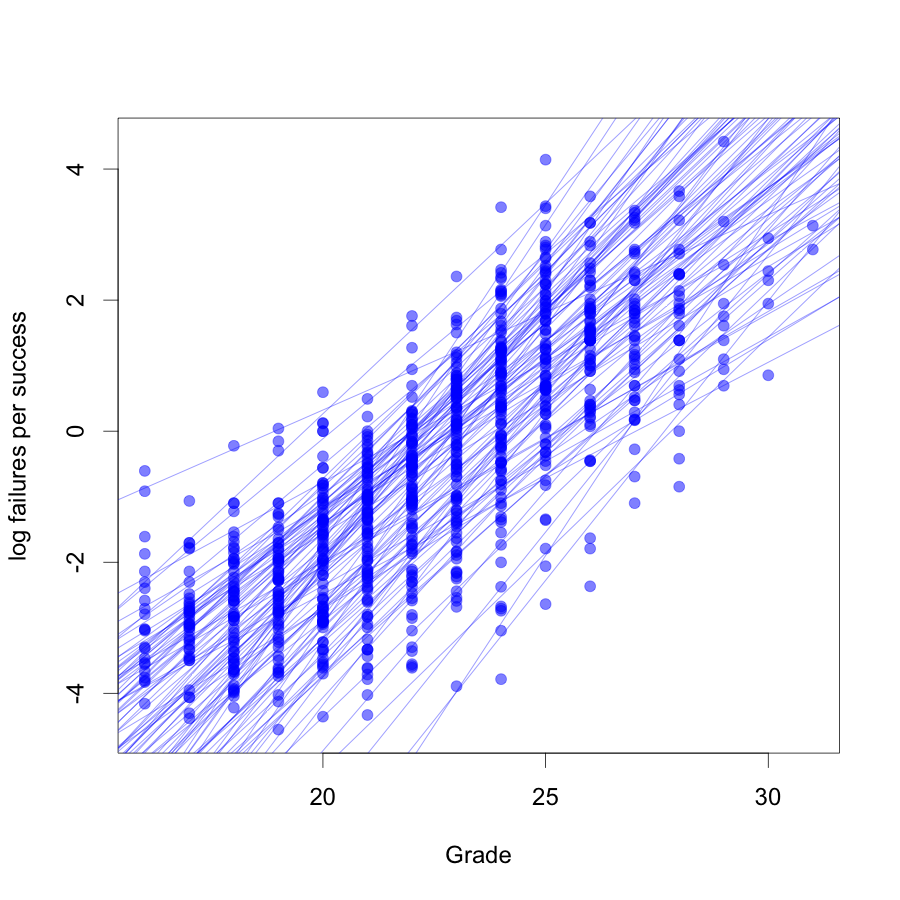
\includegraphics[width=0.9\textwidth]{../results/aus/ascents-from-2016-08-01-to-2021-08-01-minAscents30-minFails1-Sport-AU-session-regression.png}
\caption{\small The relationship between grade and the empirical log-odds-ratio of failure for the Australian climbers over a year of climbing. The point is plotted at log (\#failures / \#successes) for that grade. A regression is fit for each climber. Because there are a large number of climbers only the mean slope is reported in the main text. But it is clear that the slopes are rather consistent across climbers, despite the intercept varying by about 10 grades.}
\label{fig1}
\end{figure}


\begin{figure}
\centering
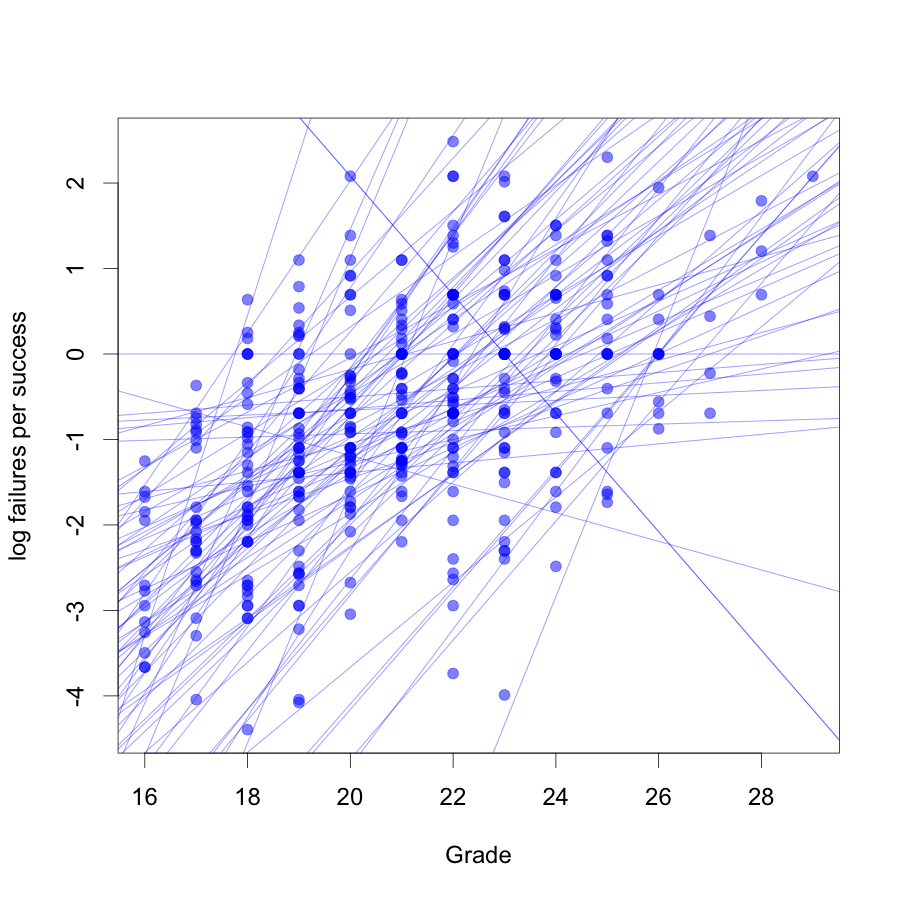
\includegraphics[width=0.9\textwidth]{../results/nz/ascents-from-2016-08-01-to-2021-08-01-minAscents30-minFails1-Sport-AU-session-regression.png}
\caption{\small The relationship between grade and the empirical log-odds-ratio of failure for the New Zealand climbers over a year of climbing. The number next to each point is the number of climbs of the grade successfully climbed over the course of the year. The point is plotted at log (\#failures / \#successes) for that grade. $m$ is the slope of the best fit, and $C_i$ is the estimated grade of the climber $i$ (i.e. the x value of the line corresponding to a log-odds-ratio of 0.}
\label{fig2}
\end{figure}

\section{Estimates of flash grade and grade scale slope assuming whole-history data available}

Figure \ref{aus_ascents_by_attempt} shows the estimated ``flash grade'' through time plot between August 2016 and July 2021 inclusive for 100 climbers that fulfilled our selection criteria and who climbed predominantly in Australia. The second panel reports the posterior distribution of the $e^m$, which was jointly estimated. The posterior estimate was 2.24 (95\% HPD:  $[2.21, 2.28]$).

\begin{figure}
\centering
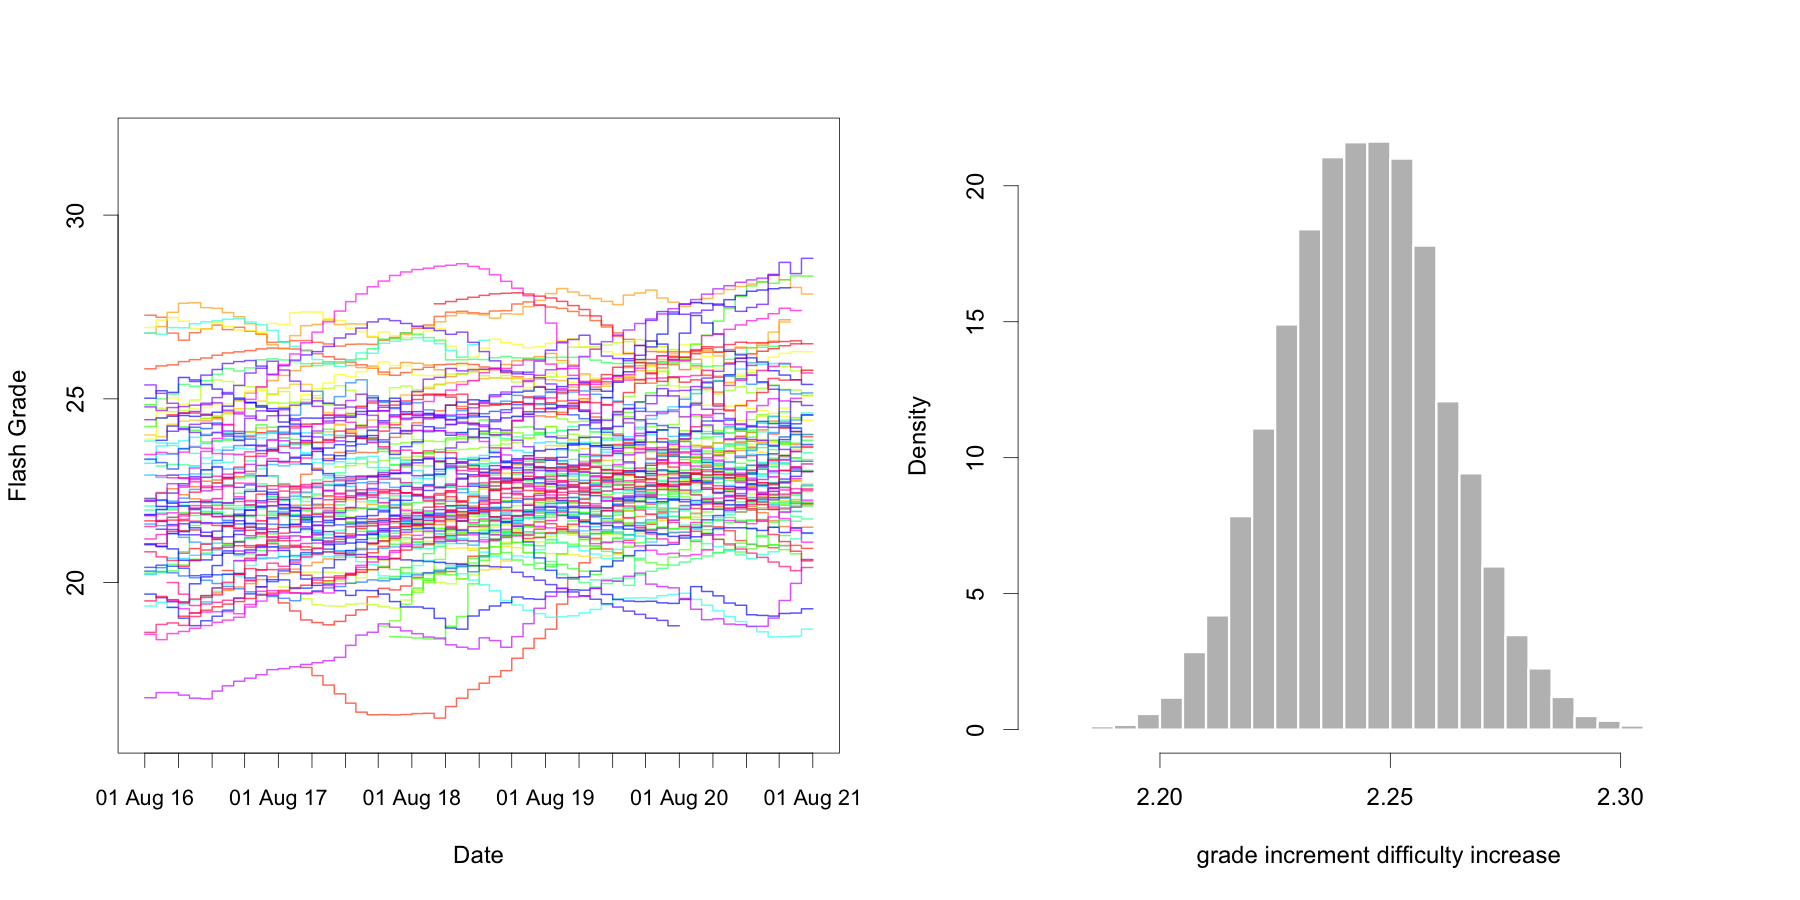
\includegraphics[width=\textwidth]{../results/aus/ascents-from-2016-08-01-to-2021-08-01-minAscents30-minFails1-Sport-AU-posterior.png}
\caption{\small The posterior estimate of each Australian climber's grade ($n=100$) through time and the posterior distribution of the proportional increase in difficulty per grade increment $d = e^m$.}
\label{aus_ascents_by_attempt}
\end{figure}

Figure \ref{nz_ascents_by_attempt} shows the estimated ``flash grade'' through time plot between August 2016 and July 2021 inclusive for 89 climbers that fulfilled our selection criteria and who climbed predominantly in New Zealand. The second panel reports the posterior distribution of the $m$ parameter which was jointly estimated.


\begin{figure}
\centering
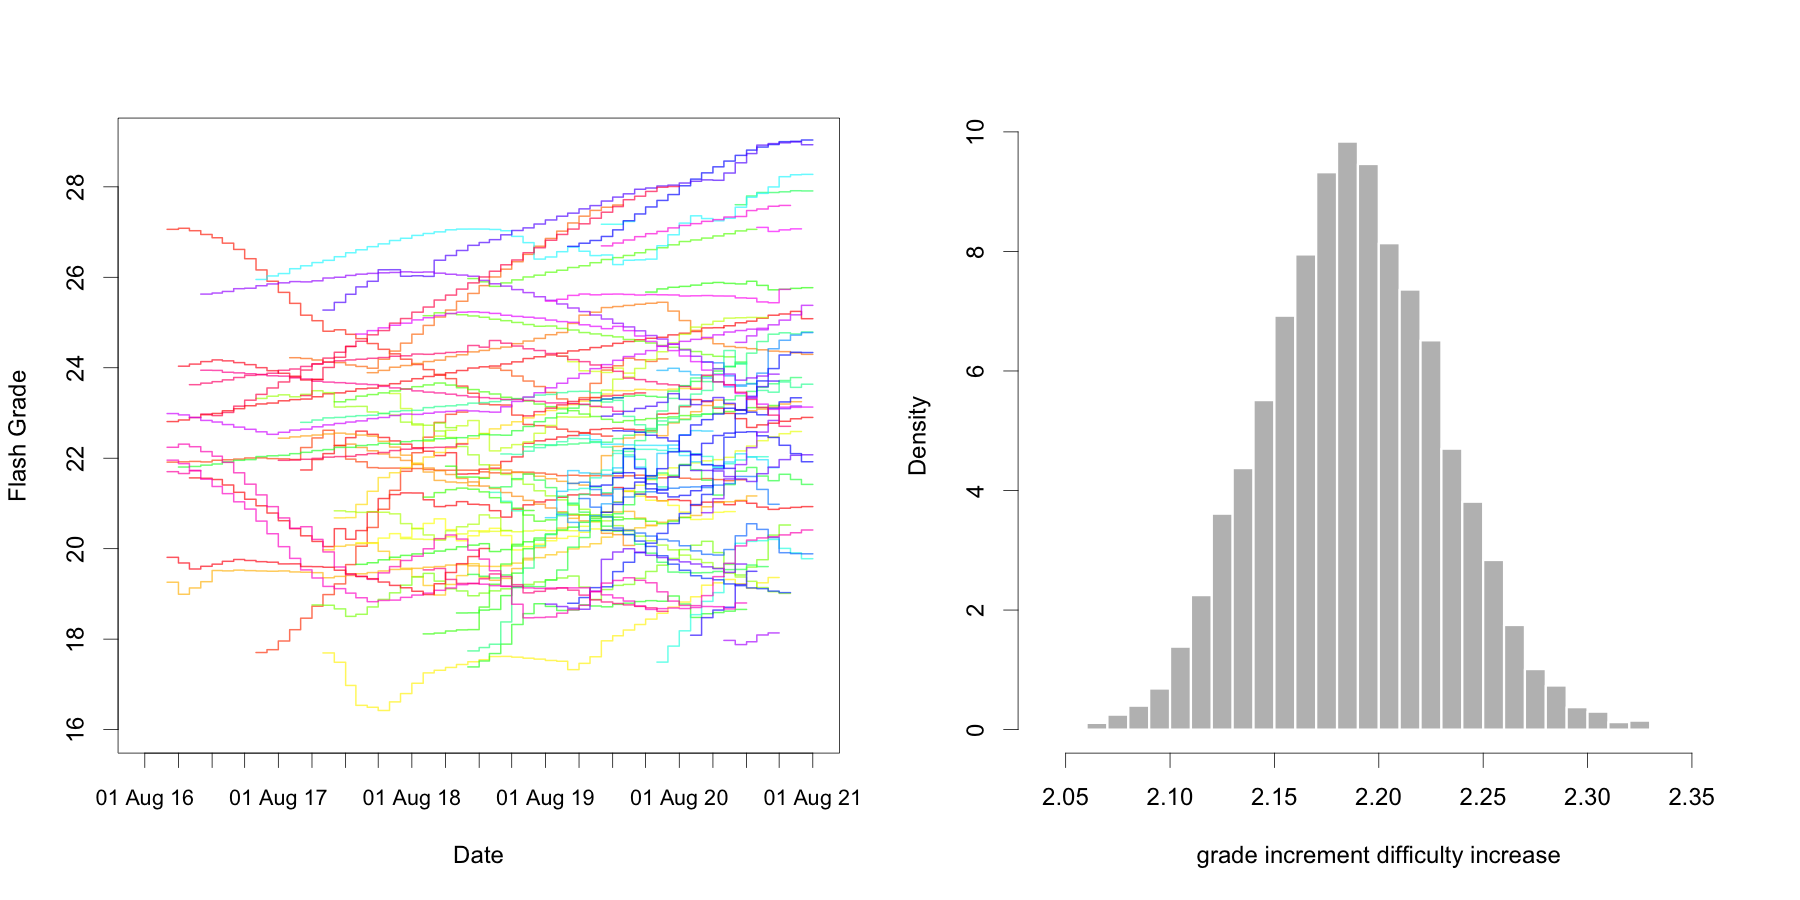
\includegraphics[width=\textwidth]{../results/nz/ascents-from-2016-08-01-to-2021-08-01-minAscents30-minFails1-Sport-AU-posterior.png}
\caption{\small The posterior estimate of each New Zealand climber's grade through time and the posterior distribution of the proportional increase in difficulty per grade increment $d = e^m$.}
\label{nz_ascents_by_attempt}
\end{figure}



\section{Interpreting whole-community ascent success data}

In 2002, Tim O'Neill published a graph of the total number of successful ascents for each grade above V9 in Australia at the time \cite{oneill2002}. He proposed a power-law relationship between the total number of ascents achieved across the climbing community $N$ and the grade $V$. He argued that if only half the climbers, on average, can climb boulder problems when the grade is increased then that suggests such boulder problems are twice as hard. We propose to fit an exponential relationship instead:

\begin{equation}
N = e^{-rx} 
\end{equation}

One of the problems with comparing the resulting slope parameter with those estimated from whole-history data is that the number of completed boulder problems of grade $x$ is the product of the number of attempts of grade $x$ and the probability of being successful on each attempt. So the ratio of the number of successes at grade $x+1$ and the number of successes at grade $x$ is:

\begin{equation}
\frac{N_A(x+1)\Pr(\textrm{success climbing } x+1 )}{N_A(x)\Pr(\textrm{success climbing } x)}
\end{equation}

where $N_A(x)$ is the number of attempts made by the community on boulder problems of grade $x$. 
Therefore the slope of the log of total successful ascents against grade will only be the same as the $m$ parameter {\it if there has been an equal number of total attempts made by the community at each grade}. This is very unlikely to be the case at the very highest grades globally. In general we might expect that very hard problems are tried less often by the community as a whole, leading to an expectation that $r$ estimated this way would be an overestimate of $m$.


%\section{Composing the grade of a route/boulder from the grades of its parts}
%
%If the probability that a climber of grade $C$ will fail to climb a route of grade ($R$) is defined by:
%
%\begin{equation}
%p_{fail} = \frac{e^{mR}}{e^{mC} + e^{mR}}
%\end{equation} 
%
%we could consider a route containing two sections, each section with it's own grade ($r_1$ and $r_2$) and recast the probability of failure like so:
%
%\begin{equation}
%p_{fail} = \frac{e^{mr_1} + e^{mr_2}}{e^{mC} + e^{mr_1} + e^{mr_2}}
%\end{equation} 
%
%Continuing in this vein we could break the route down into its $K$ constituent moves so that:
%
%\begin{equation}
%p_{fail} = \frac{\sum_{i=1}^{K}e^{mr_i}}{e^{mC} + \sum_{i=1}^{K}e^{mr_i}}
%\label{compose}
%\end{equation} 
%
%where for consistency we would require
%
%\begin{equation}
%e^{mR} = \sum_{i=1}^{K}e^{mr_i}
%\end{equation} 
%
%This provides a mathematical basis for composing the grade of a climb from the scaled logarithm of the sum of the grades of its constituent parts:
%
%\begin{equation}
%R = \frac{1}{m} \ln \left(\sum_{i=1}^{K}e^{mr_i}\right)
%\end{equation} 
%
%As an example, take $m=1$. Then if a route involved climbing two back-to-back routes that were individually graded at Ewbank 25 then the grade of the combined route is expected to be:
%
%\begin{equation}
%R = \frac{1}{m} \ln \left(e^{mr_1} + e^{mr_2}\right) = \ln \left(2 * e^{25}\right) \approx 25.7
%\end{equation} 
%
%This should be considered a minimum estimate of the grade of the combined route, as it assumes that the climber doesn't get fatigued in the course of climbing the first section, or that (equivalently) a full rest (both mental and physical) is possible in between the two sections, without weighting the rope.
%
%The difference between this computed grade and the actual grade gives an estimate of the fatigue factor (e.g. increased ``pump'', decreased power, and increased mental fatigue) caused by the first part of the route. One would expect that this model would exhibit the smallest fatigue factors when applied to boulder problems. 
%
%\subsection*{Estimating the fatigue factor for link-up boulder problems}
%
%
%For example, Adam Ondra proposed a grade of V16/8C+ for the boulder problem known as Brutal Rider, which is a link up of two individual boulder problems climbed back to back: Brutus (8A+/8B or V12/V13) and Ghost Rider (8C/V15). The theoretical grade should be:
%
%\begin{equation}
%R = \ln \left(e^{12.5} + e^{15}\right) = 15.34
%\end{equation} 
%
%Yet the grade assigned is 16. The difference between the estimate 15.34 and the range that would be assigned 16 (15.5-16.49)  is 0.16-1.15 of a grade. We assumed that this difference comes from fatigue (the rest Ondra could take between the two boulder problems is no-hands but strenuous and only about 20 seconds long). The discrepancy could be partially caused by inaccuracies in the grading of the subproblems (maybe Ghost Rider is already 15.25 for example).
%
%\begin{table}
%\centering
%\begin{tabular}{| c | c | c | c | c | c |}
%  \hline			
%  {\bf Boulder } & {\bf V-grade} & {\bf part 1} & {\bf part 2} & {\bf Expected} & {\bf Fatigue factor } \\
%  \hline			
%  Brutal Rider & 16 & 12/13 & 15 & 15.34 & 0.66 [0.16-1.15]\\
%  Vampire Dagger & 11 & 9 & 9 & 10.16 & 0.84 [0.34-1.33]\\
%  L'homme Obu & 11 & 8 & 10 & 10.44 & 0.56 [0.06-1.05]\\
%  Bursting & 8 & 5 & 7 & 7.44 & 0.56 [0.06-1.05]\\
%  \hline  
%\end{tabular}
%\caption{The summary of calculated fatigue factors for a selection of well-known boulder problems. }
%\label{table2}
%\end{table}



\bibliography{climbing}

\end{document}
